En esta sección se va a explicar la metodología utilizada a lo largo del proceso de desarrollo de software. Lo primero cabe destacar que se va a utilizar una herramienta de gestión de proyectos, de código abierta y gratuita. La idea del uso de esta herramienta tiene que ver con la metodología de desarrollo que se va a llevar a cabo durante el transcurso de este trabajo de fin de grado. La metodología usada en cuestión es Kanban. A continuación hay una breve descripción para las personas que la desconozcan. 

\subsubsection{Kanban}

El modelo de proceso que se va a utilizar para el desarrollo del proyecto será Kanban. Se trata de un modelo similar a Scrum pero con unas directivas más flexibles. La idea en la que se basa Kanban es visualizar el flujo de trabajo mediante segmentos o estados definidos, representados por columnas en un tablero. Los segmentos que se suelen utilizar son los siguientes:

\begin{itemize}
    \item \textbf{Nuevas}: (new) son las tareas que se han ido añadiendo al backlog, el backlog es la lista de tareas e historias de usuario que se crean en el proyecto. Las nuevas tareas se crean por defecto en el estado de nuevas. 
    
    \item \textbf{Preparado}: (ready) tareas que aún no han comenzado, pero que lo harán en algún momento del futuro. En esta columna se pondrán las siguientes tareas a ser desarrolladas. 
    
    \item \textbf{En desarrollo}: (in progress) a esta columna también se le llama WIP (Work in Progress). La conforman las tareas que se están llevando a cabo en un instante de tiempo determinado. 
    
    \item \textbf{Bloqueadas}: en la que se mostrarán las tareas que están siendo bloqueadas debido a razones externas. Por ejemplo la tarea depende de la finalización de otra actividad, o tenemos que preguntar alguna duda al cliente, o se ha caído un servicio del que depende la tarea. En este caso concreto, no tendremos columna de bloqueadas, porque la herramienta las muestra de otra manera, pero es común que en los tableros kanban aparezca dicha columna. 
    
    \item \textbf{En revisión}: (in review) en esta columna se dispondrán las actividades que están acabadas pero pendientes de revisión por parte de otros compañeros. Las actividades de esta columna tendrán un enlace a la PR asociada para ganar una mayor continuidad del trabajo. Como este trabajo va a ser desarrollado por una única persona, o como mucho el trabajo será supervisado por el tutor, no contaremos con dicha columna en nuestro tablero. 
    
    \item \textbf{Preparadas para probar}: tareas que han sido realizadas y aprobadas y que tienen que ser testeadas, en el caso de tener una CI/CD, es conveniente tener esta columna. La idea del proyecto es contar con un CI/CD, por lo menos cuando se tenga el suficiente código desarrollado como para que se permita. 
    
    \item \textbf{Hechas}: (done) tareas completadas, dicha columna se irá vaciando y las tareas se pasarán a archivadas, simplemente para que no se sature la vista de la columna de Hecho.
\end{itemize}

El principio básico de Kanban es que separando las tareas del proyecto en estos segmentos se garantiza que el trabajo del equipo se visualice de forma clara. Además, permite que el workflow se unifique en un solo lugar y que se identifiquen y resuelvan inmediatamente todos los factores que lo bloqueen y de los que dependan.

Cada elemento de trabajo en Kanban se representa en una tarjeta distinta y esta se coloca en una columna para indicar su posición en el flujo de trabajo. Estas tarjetas son las llamadas User stories, que son tareas inicialmente sencillas, que más adelante se subdividen en subtareas para su implementación. Estas tarjetas proporcionan visibilidad a todo el equipo sobre quién está a cargo de qué elementos, la descripción del trabajo y una estimación de la duración del mismo. A mayores (en tablas virtuales Kanban) se suelen añadir capturas de pantalla y otros datos técnicos de valor para el destinatario de la asignación. También en las tarjetas Kanban se permite una estimación de la dificultad de implementación de la actividad, además de una estimación del tipo de tareas que va a desempeñar. La estimación de la dificultad se hace siguiendo la serie de fibonacci. Esto se hace así porque la complejidad normalmente crece en el mismo orden que esta serie. 

El segmento central (WIP) y, opcionalmente, el resto de segmentos, tienen especificado un límite de tareas que pueden contener en un instante. Un elemento no podrá pasar a la siguiente columna a no ser que haya espacio disponible. De esta forma se evita el exceso de trabajo activo sin necesidad de sprints que definan la cantidad de tareas asignadas. Normalmente el WIP para cada uno de los integrantes del equipo será de 2 tareas como máximo. 

Kanban nos proporciona una reducción de los cuellos de botella. Cuantos más elementos de trabajo haya en curso más se cambia el contexto, por lo tanto una de las cosas que propone Kanban es limitar la cantidad de trabajo en curso. La limitación del trabajo hace que resalten los cuellos de botella.

Otra de las ventajas es una mejor estimación de las entregas futuras debido a que se puede ver cuánto tarda en viajar una actividad de trabajo a través del workflow desde que comienza hasta que se envía.

los principios básicos de Kannban se asientan en los principios básicos del manifiesto ágil \cite{manifiestoAgil} y en los principios seguidos por Scrum. 

A nivel personal, las referencias de la empresa Atlassian \cite{atlassian} para gestión de proyectos y para información de metodologías me parecen muy buenas, tanto para Kanban \cite{kanbanAtlassian} como para Scrum \cite{scrumAtlassian}. 

En nuestro caso, la herramienta que vamos a utilizar para tener un poco de control en el proyecto y seguir esta aproximación a Kanban, va a ser Taiga, que se describe mas adelante de manera breve. Por ejemplo, la empresa Atlassian, tiene su propio software de control de proyectos grupales ágiles, llamado Jira \cite{jiraAtlassian}, usado por grandes compañías a nivel mundial. 

Ahora que hemos descrito de manera breve, la metodología que vamos a utilizar, vamos a hablar de las tecnologías principales que se van a utilizar en este proyecto de software. 

\subsubsection{Gitflow}
 
En los proyectos de software principalmente se trabaja desarrollando código y una vez completados los módulos principales, se van mejorando. Dentro de estos proyectos hay ciertas maneras y formas de trabajar de manera adecuada sobre dicho código. Las diferentes formas de desarrollo que un proyecto y miembros del equipo siguen a la hora del desarrollo del código se denomina Gitflow. 

Originalmente el termino de Gitflow \cite{gitflow} fue acuñado por Vincent Driessen en Nvie. Lo que esta metodología define es la creación de un conjunto de ramas especificas, cada una con unas reglas determinadas a la hora de programar con el objetivo de tener un control de las versiones de código del proyecto junto con un control total sobre las versiones finales o de prueba que el equipo va consiguiendo. 

El Gitflow es ideal para los proyectos en los que hay marcas de tiempo bastante fuertes. No se introducen conceptos nuevos a la hora del control del código. Simplemente se marca un patrón bien definido, junto con una serie de roles para cada una de las ramas. Con esto conseguiremos los objetivos de tiempo con una mayor facilidad y rapidez. 

El patrón definido por Gitflow no es demasiado complejo, para proyectos pequeños es incluso mas tedioso aplicarlo correctamente que simplemente empezar a desarrollar código e ir actualizando el repositorio. Pero incluso para equipos pequeños, de 2 o 3 personas, es muy útil e impide problemas en el futuro derivados de un uso incorrecto de las herramientas de control de versiones. 

Primero vamos a mostrar un poco como es el patrón original al completo y luego vamos a explicar la adaptación que yo voy a llevar a cabo en este proyecto, ya que en mi opinión no es necesario aplicar el patrón completo al 100\%. 

\subsubsection*{Patrón original}

Este patron nos define un conjunto de ramas sobre los que vamos a trabajar:
\begin{itemize}
    \item \textbf{Master}: la rama master es la que lleva el control de las versiones finales con capacidad suficiente como para existir por ellas solas y que están en el entorno de producción del cliente. Normalmente la rama master no va nunca sola, y en este modelo se encuentra bloqueada, es decir no se pueden hacer commits (cambios) en ella de manera directa, para cambiar esta rama siempre tiene que haber una solicitud de cambio de otra rama. 
    \item \textbf{Develop}: en esta rama se van desarrollando las diferentes partes de la aplicación. Por ejemplo imaginemos que estamos desarrollando un servicio fullstack para una empresa, en develop es donde se verian reflejados todos y cada uno de los cambios, pero como veremos mas adelante, no siempre se hacen los cambios directamente sobre develop. 
    \item \textbf{Features}: para llevar un control de grano mas fino acerca de los diferentes cambios, quien los hace y cuando, para cada una de las partes principales de la aplicación se suele sacar una rama llamada feature. Por ejemplo, continuando con el desarrollo de la aplicación fullstack, podríamos sacar una rama develop para el front y una rama develop para el back y a su vez, ramas de funcionalidad de cada una de las ramas de desarrollo de front y de back. Por ejemplo una rama valida de funcionalidad para el back seria login, en la que se implementarían las funciones de login de la aplicación. 
    \item \textbf{Hotfix}: estas ramas son ramas que se sacan directamente de master y se acaban fusionando con master, porque aplican cambios importantes que arreglan fallos graves en el entrono de producción que necesitan ser arreglados en el menor tiempo posible. 
\end{itemize}

Podemos observar este patrón al completo en la siguiente figura: 

\begin{figure}[H]
    \centering
    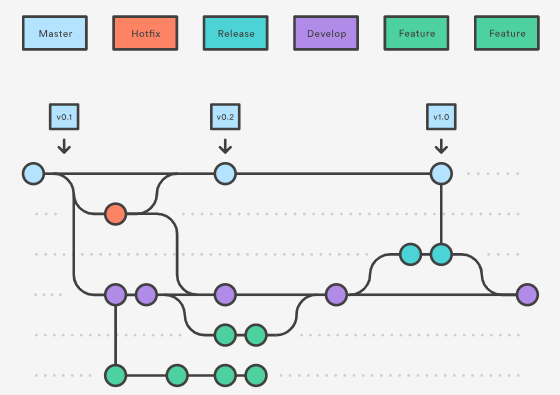
\includegraphics[scale=0.7]{imagenes/fundamentosHerramientas/gitflow.png}
    \caption{Patrón completo}
    \label{fig:gitflowCompleto}
\end{figure}

\subsubsection*{Patrón derivado}

En mi caso se va a seguir un patrón mas flexible ya que no es un proyecto demasiado grande y en mi opinión no hace falta cumplir con el patrón al completo. La idea es la siguiente: 
\begin{itemize}
    \item \textbf{Master}: rama en la que existirán las versiones principales y funcionales de la aplicación. Cada una de las diferentes versiones que se consideren finales se etiquetaran con un tag del tipo: V1.0.0. Esta rama estará bloqueada y solo se podrán realizar cambios mediante peticiones de cambio. 
    \item \textbf{Features}: ramas de funcionalidad, son sacadas directamente desde master y desarrollan las diferentes funcionalidades que tendrá la aplicación. Se fusionaran directamente con master cuando se considere necesario. 
    \item \textbf{Hotfix}: las ramas de hotfix son necesarias en todos los proyectos. Siempre surgen problemas que hay que resolver en el menor tiempo posible sin tener en cuenta el resto de funcionalidades que se están implementando en el momento. No serán las mas comunes, pero alguna rama de este tipo habrá en el proyecto. 
\end{itemize}

\textcolor{red}{incluir un diagrama de la modificación que he seguio yo}
